\documentclass[]{article}  % list options between brackets
\usepackage{graphicx}              % list packages between braces
\usepackage{url}
\usepackage{color}
\usepackage{amsfonts}
\usepackage{algpseudocode}
\usepackage{hyperref}

% type user-defined commands here

\begin{document}

\title{AdaBoost Notes}   % type title beTrending Predictiontween braces
\author{Yang Gu@ Scopely}         % type author(s) between braces
\maketitle
\setcounter{tocdepth}{2}

\pagenumbering{roman}
\tableofcontents
\newpage
\pagenumbering{arabic}


\section{Introduction}

AdaBoost or Adaptive Boosting, is an algorithm used for generating strong classifiers out of weak classifiers. For a given input $x$ each expert classifier $k_j$ can emit an opinion $k_j(x)\in \{-1,1\}$, and the final decision of the committee $K$ of experts is sign$(C(x))$, the sign the weighted sum of expert opinions, where
\[
C(x) = \sum_j^L \alpha_j k_j (x),
\]
where constants $\alpha_j$ is the weight we assign to the opinion of the $j$th expert in the committee. 

The process of AdaBoost consists three steps: 1) scouting prospective experts, 2) drafting them, and 3) assigning a weight to their contribution to the team~\cite{tutorial}.

\section{AdaBoost}

\subsection{Scouting}

Scouting is done by testing the classifiers in the pool using a training set $T$ of $N$ multidimensional data points $x_i$. For each point $x_i$ we have a row $i$ built in matrix with misses (with a 1) and hits (with a 0) of each classifier. Column $j$ is reserved for the $j-th$ classifier in the pool:

\begin{table}[htdp]
\caption{Scout table of classifiers}
\begin{center}
\begin{tabular}{c|cccc}
 & 1 & 2 & $\cdots$ & L\\
 \hline
$x_1$ & 0 & 1 & $\cdots$ & 1\\
$x_2$ & 0 & 0 & $\cdots$ & 1\\
$\vdots$ & $\vdots$ & $\vdots$ &  & $\vdots$ \\
$x_N$ & 0 & 0 & $\cdots$ & 0
\end{tabular}
\end{center}
\label{default}
\end{table}%

The main idea of AdaBoost is to proceed systematically by extracting one classifier from the pool in each of $M$ iterations. At beginning, all elements ($\alpha_j$) are assigned the same weight (e.g., $1$). As the drafting progresses, the more difficult examples, that is, those where the committee still perform badly, are assigned larger and larger weights. The best "team players" are those which can provide new insights to the committee. Classifiers being drafted should complement each other in an optimal way.

\subsection{Drafting}

In each iteration, we need to rank all classifiers, so that we can select the current best out of the pool. At the $m$-th iteration we have already included $m-1$ classifiers in the committee and we want to draft the next one. The current linear combination of classifiers is 
\[
C_{m-1}(x) = \sum_j^{m-1} \alpha_j k_j(x)
\]
and we want to extend it to
\[
C_m(x) = C_{m-1}(x) + \alpha_m k_m(x).
\]
At the first iteration ($m=1$, $C_0$ is the zero function. We define the total cost, or total error, of the extended classifier as the exponential loss

\[
E = \sum_{i=1}^N e^{-y_i C_{m}(x_i)} = \sum_{i=1}^N e^{-y_i (C_{m-1}(x_i) + \alpha_m k_m(x_i))}
\]
where $y_i \in \{-1,1\}$. 

If the committee's opinion (the sign) is different (a miss) with the label, e.g. $C_m(x_i) = \beta, y_i = -1$ where $\beta > 0$ or vise versa, 
\[
- y_i C_m = - (-1 \cdot \beta) = \beta,
\]
the expert pool is charged by a cost $e^\beta$.

If the committee's opinion (the sign) is the same (a hit) as the label, e.g. $C_m(x_i) = -\beta, y_i = -1$ or vise versa, 
\[
- y_i C_m = - (-1 \cdot -\beta) = -\beta,
\]
the expert pool is charged by a cost $e^{-\beta}$. Note that $e^{-\beta} < e^{\beta}$, so that misses are more heavily penalized than hits. 

Since our intention is to draft $k_m$ we rewrite the above expression as
\begin{equation}\label{w1}
E = \sum_{i=1}^N w_i^{(m)} e^{-y_i \alpha_m k_m(x_i)},
\end{equation}
where 
\begin{equation}
w_i^{(m)} = e^{-y_i C_{m-1} (x_i)},
\end{equation}
In the first iteration $w_i^{(1)} = 1 $ for $i=1,2,\cdots, N$. During later iterations, the vector $w^{(m)}$ represents the weight assigned to each data point in the training set at iteration $m$. We can split the sum in Eq.~\ref{w1} into two sums

\begin{eqnarray}
E &=& \sum _{y_i = k_m(x_i)} w_i^{(m)} e^{-\alpha_m} +  \sum _{y_i \neq k_m(x_i)} w_i^{(m)} e^{\alpha_m} \\
 & =& W_c e^{-\alpha_m} + W_e e^{\alpha_m} \label{w3}
\end{eqnarray}
which means that the total cost is the weighted cost of all hits plus the weighted cost of all misses.

Minimizing $E$ is equivalent to minimizing $e^{\alpha_m}E$ for a fixed $\alpha_m$,
\begin{eqnarray}
e^{\alpha_m}E &= & W_c + W_e e^{2\alpha_m}\\
 & = & (W_c + W_e) + W_e ( e^{2\alpha_m} -1)\\
 & = & W + W_e ( e^{2\alpha_m} -1)
\end{eqnarray}

$W=W_c + W_e$ is the total sum of the weights of all data points, that is, a constant in the current iteration. The right hand side of the equation is minimized when at the $m$-th iteration we pick the classifier with the lowest total cost $W_e$ (we know $e^{2\alpha_m} > 1$). The next Draftee, $k_m$, should be the one with the lowest penalty given the current set of weights.

\subsection{Weighting}

Having picked the $m$-th member of the committee we need to determine its weight $\alpha_m$. From Eq~\ref{w3} we see that (note $de^x/dx = e^x$)
\[
\frac {dE}{d\alpha_m} = -W_ce^{-\alpha_m} + W_e e^{\alpha_m}
\]
Setting the above equation to 0 and multiplying by $e^{\alpha_m}$ we obtain
\[
-W_e + W_e e ^{2\alpha_m} = 0
\]
The optimal $\alpha_m$ is thus:
\[
\alpha_m = \frac{1}{2} \ln \left(\frac{W_c}{W_e}\right) = \frac{1}{2} \ln \left(\frac{1-e_m}{e_m}\right) ,
\]
where $e_m$ = $W_e/W_m$, is the percentage rate of error given the weights of the data points. Since the percentage is invariant if we normalize the weight, normalizing the weights of data at each iteration is irrelevant.

We proceed to get the recursive update equations:

\begin{eqnarray*}
e^{-\alpha_m} &=& e^{-\frac{1}{2} \ln \left(\frac{1-e_m}{e_m}\right)}\\
&=& (e^{\ln \left(\frac{1-e_m}{e_m}\right)})^{-\frac{1}{2}}\\
&=& \sqrt{\frac{e_m}{1-e_m}}
\end{eqnarray*}

\begin{eqnarray*}
e^{\alpha_m} &=& e^{\frac{1}{2} \ln \left(\frac{1-e_m}{e_m}\right)}\\
&=& (e^{\ln \left(\frac{1-e_m}{e_m}\right)})^{\frac{1}{2}}\\
&=& \sqrt{\frac{1-e_m}{e_m}}
\end{eqnarray*}

\begin{eqnarray*}
w_i^{(m+1)} &=& e^{-y_i C_m(x_i)}\\
&=& e^{-y_i (C_{m-1}(x_i) + \alpha_m k_m(x_i))}\\
&=& e^{-y_i C_{m-1}(x_i)} \cdot e^{-y_i \alpha_m k_m(x_i)}\\
&=& w_i^{(m)} e^{-y_i \alpha_m k_m(x_i)}
\end{eqnarray*}

\begin{equation}\label{weight-update}
w_i^{(m+1)}=\left\{
\begin{array}{ccc}
w_i^{(m)} e^ {-\alpha_m}=w_i^{(m)}\sqrt{\frac{e_m}{1-e_m}} ,  & y_i = k_m(x_i) & hit\\
w_i^{(m)} e^{\alpha_m}=w_i^{(m)}\sqrt{\frac{1-e_m}{e_m}}, & y_i \neq k_m(x_i) & miss
\end{array} \right.
\end{equation}

\subsection{Pseudocode}
Given a training set $T$ of data points $x_i$ and their labels $y_i$ in a two class problem, we assign initial weights $w_j^{(1)}=1$ to all data points $x_i$. We perform $M$ iterations.

For $m=1$ to $M$
\begin{enumerate}

\item Select and extract from the pool of classifiers the classifier $k_m$ which minimizes 
\[
W_e = \sum _{y_i\neq k_m(x_i)}w_i^{(m)}
\]
\item Set the weight $\alpha_m$ of the classifier to 
\[
\alpha_m = \frac{1}{2} \ln \left(\frac{W_c}{W_e}\right) 
\]

\item Update the weights of the data points for the next iteration. If $k_m(x_i)$ is a miss, set
\[
w_i^{(m+1)} = w_i^{(m)} e^{\alpha_m}=w_i^{(m)}\sqrt{\frac{1-e_m}{e_m}} 
\]
otherwise 
\[
w_i^{(m+1)} =w_i^{(m)} e^ {-\alpha_m}=w_i^{(m)}\sqrt{\frac{e_m}{1-e_m}}
\]
\end{enumerate}

\section{Example}

Define a two-class problem in the plane:
\begin{itemize}
\item class 1: points in circle $x^2+y^2 < 1$

\item class 2: points not in circle and in box 
\begin{itemize}
\item $-2\leq x \leq 2 $ and
\item $-2 \leq y \leq 2 $ and
\item$x^2 + y^2 > 1$ 
\end{itemize}
\end{itemize}

which includes a circle of points inside a square. We will build a strong classifier out of a pool of $L$ (10 or 100) randomly generated linear discriminates of the type sign$(ax_1+bx_2+c)$. 

\subsection{Data Points}

Below python code generates 1000 data points for each class.
\begin{verbatim}
N = 1000
def unif(n):
    vec = []
    while len(vec) < n:
        vec.append(uniform(-1,1))
    return vec

def generate_class(label=1):
    X = []
    while len(X) < N:
        x,y = unif(2)
        if label ==1 and x**2 + y**2 >= 1: continue
        if label ==-1:
            x *= 2; y*= 2
            if x**2 + y**2 < 1: continue
        X.append([x,y])
    return X
\end{verbatim}

\begin{figure}[h]
\begin{center}
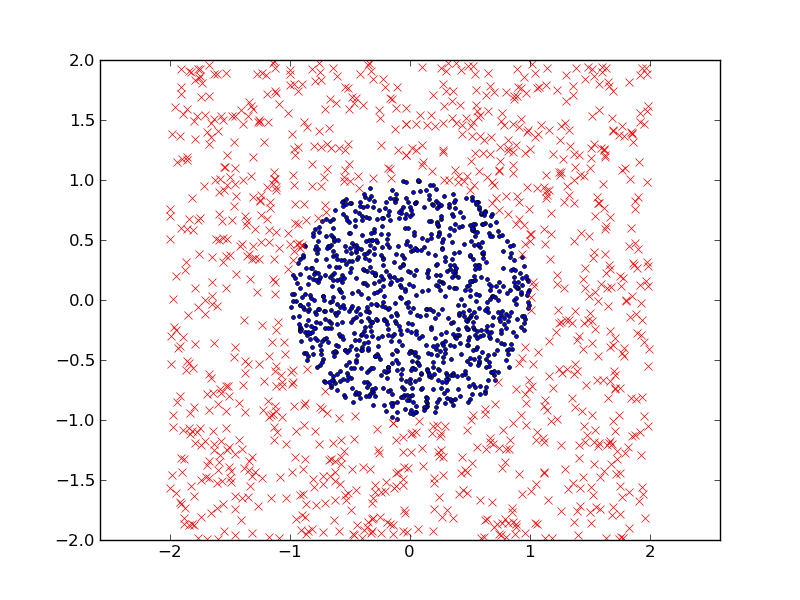
\includegraphics[scale=.6]{plane.png}\label{fig:axis}
\end{center}
\caption{The data plot of the two-class problem. Blue dots are in class 1 and red crosses are in class 2. }
\end{figure}%%%%%%%%%%%

\subsection{Weak Classfifiers}
We randomly generate $L$ linear discriminants using below code:
\begin{verbatim}
L = 10
def generate_classifiers():
    C = []
    while len(C) < L:
        a,b,c = unif(3)
        C.append([a,b,c])
    return C
\end{verbatim}

\begin{figure}[h]
\begin{center}
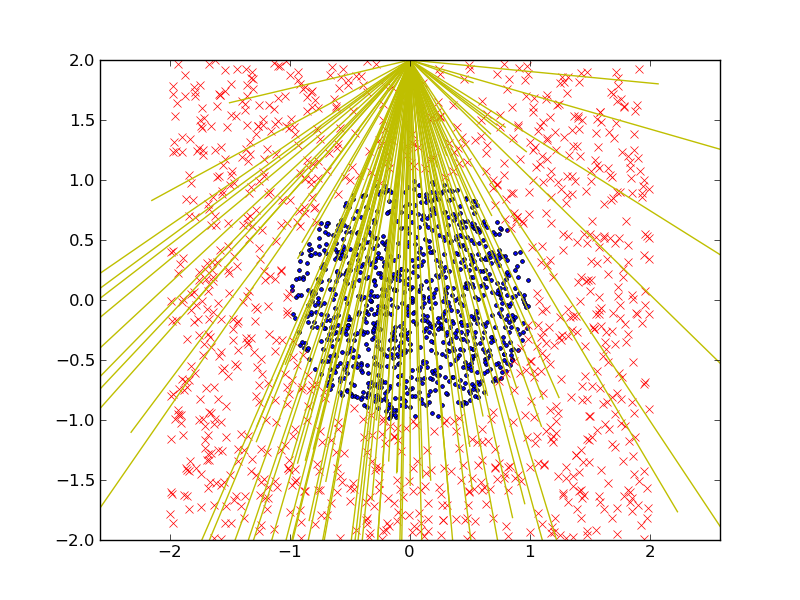
\includegraphics[scale=.6]{plain_with_c.png}\label{fig:axis}
\end{center}
\caption{The data plot of the two-class problem. Blue dots are in class 1 and red crosses are in class 2. The yellow lines are linear classifiers.}
\end{figure}%%%%%%%%%%%

To get predictions from the linear classifiers:

\begin{verbatim}
def is_prediction_hit(classifier, data, label):
    a,b,c = classifier
    x, y = data
    if linear(a,b,c,x,y) > 0:
        pred = 1
    else:
        pred = -1
    return pred == label
\end{verbatim}

\subsection{Scout}
Assuming class 1 are labeled with `True' and class 2 are labeled with `False' in our data. We generate our scout table with below codes:
\begin{verbatim}
X1 = generate_class(1)
X2 = generate_class(-1)
C = generate_classifiers()
pred = fill_scout()

def fill_scout():
    pred = {}
    for j, classifier in enumerate(C):
        pred[j] = []
        for i,data in enumerate(X1):
            pred[j].append(is_prediction_hit(classifier, data, 1))
        for i,data in enumerate(X2):
            pred[j].append(is_prediction_hit(classifier, data, -1))
    return pred
\end{verbatim}

\subsection{Initialization}
\begin{verbatim}
w = [1.0]*(2*N)
alpha = [0]*L
in_committee = set()
\end{verbatim}

\subsection{Training}
\begin{verbatim}
def get_draftee(pred):
    min_We = 1e100
    min_W = 1e100
    min_classifier = -1
    for j in range(L):
        if j in in_committee: continue
        We = 0
        W = 0
        for i,prediction in enumerate(pred[j]):
            W += w[i]
            if not prediction:
                We += w[i]
        if We < min_We:
            min_classifier = j
            min_We = We
            min_W = W
            
    em = float(min_We)/min_W
    print min_We, min_W
    alpha[min_classifier] = .5*log((1-em)/em)
    in_committee.add(min_classifier)
    
    for i in range(2*N):
        if not pred[min_classifier]:
            w[i] *= ((1-em)/em)**.5
        else:
            w[i] *= (em/(1-em))**.5 
\end{verbatim}

\subsection{Results}

Test code:

\begin{verbatim}
def test(X, y):
    cnt = 0
    for i,data in enumerate(X):
        pred = 0
        for j, classifier in enumerate(C):
            if is_prediction_hit(classifier, data, y):
                pred += alpha[j]
            else:
                pred += -alpha[j]
        if (pred > 0 and y > 0) or (pred < 0 and y < 0): cnt += 1
    return cnt
        
def testAll(X1, X2):
    cnt = 0
    cnt += test(X1, 1)
    cnt += test(X2, -1)
    print float(cnt)/2/N
    
T1 = generate_class(1)
T2 = generate_class(-1)

testAll(X1,X2)
testAll(T1,T2)
\end{verbatim}
Training/Testing error : percentage of wrongly classified points

\begin{table}[htdp]
\caption{Training and Testing error }
\begin{center}
\begin{tabular}{c|c|c|c|c}

number of classifiers & 10 & 20 & 50 & 100\\
\hline
Train Error \% & 13.7 & 4.6 & 1.45 & 0\\
Test Error\% & 13.85 & 5.0 & 2.3 & 0
\end{tabular}
\end{center}
\label{default}
\end{table}%

\begin{figure}[h]
\begin{center}
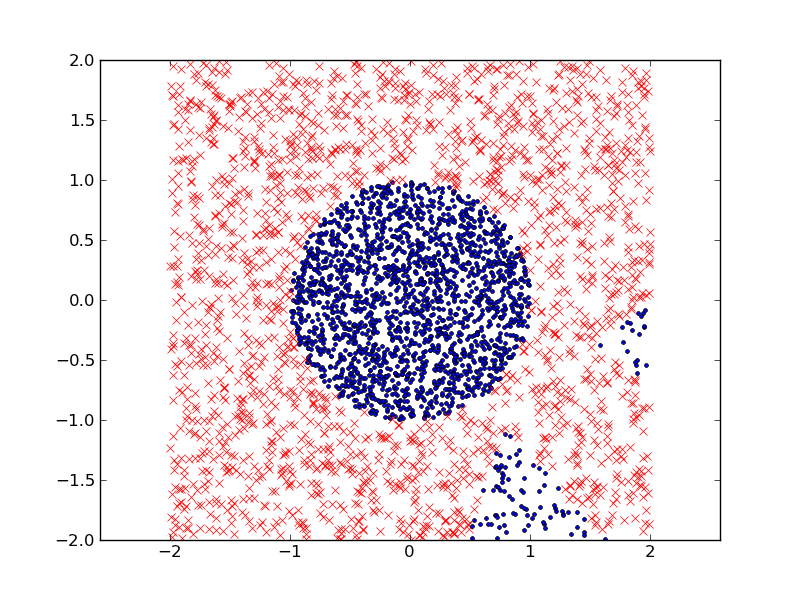
\includegraphics[scale=.6]{10c.png}\label{fig:axis}
\end{center}
\caption{Predicted class labels in testing with 10 classifiers with some wrong labels. It is very clear that those error appears where we lack training examples. }
\end{figure}%%%%%%%%%%%

\begin{thebibliography}{9}

\bibitem{tutorial} Baul Rojas, \emph{AdaBoost and the Super Bowl of Classifiers: A tutorial introduction to Adaptive Boosting}, \url{http://www.inf.fu-berlin.de/inst/ag-ki/adaboost4.pdf}


\end{thebibliography}
\end{document}